\chapter{Pruebas realizadas}

En este capítulo se detallan las pruebas realizadas sobre las distintas herramientas y editores, así como su instalación y la integración de varias de ellas formando una única solución.

El objetivo de estas pruebas no es otro que el de obtener la solución idónea y no tener que arrepentirnos más tarde de la opción escogida, con la pérdida de tiempo que eso conllevaría. Además, de esta forma nuestro editor será una solución mucho más madura debido a este tiempo que emplearemos en reflexionar sobre lo que hemos llamado state-of-the-art.

Cómo ya dijimos previamente, no se trata de reinventar la rueda. Muchos de los editores analizados dan soluciones muy buenas al problema del editor WYSIWYG, además de ser proyectos estables con algunos años en desarrollo. 

Lo mejor de todo es que la mayoría de las herramientas analizadas se distribuyen bajo licencias de software libre, lo que nos da libertad de ejecutar, copiar, distribuir, y estudiar el mismo, e incluso modificar el software y distribuirlo modificado. 

\section{Prueba de editores}
\subsection{CKEditor}
\section{Prueba MathJax}
\section{Pruebas Soporte Fórmulas}
\subsection{Generador de fórmulas AJAX con tex2png}
Se implementó un generador de fórmulas en el que mientras el usuario escribe el código {\LaTeX} se generan peticiones al servidor que va enviando al cliente imágenes, renderizando el código escrito. 

El problema de esta solución es el gran número de imágenes (temporales) generadas en el servidor las cuales posteriormente deberían de ser eliminadas.

Otro problema acontecido fué la generación errónea de imágenes por parte de tex2png, por ellos nos planteamos usar la herramienta texvc.

\subsection{Generador de fórmulas usando MathJax y texvc}

\section{Pruebas de integración}
\subsection{NicEdit + MathJax}

Como primera aproximación de nuestro editor WYSIWYG se pensó en la unificación del editor NicEdit junto con MathJax. Dicho editor fué bautizado como Nax y como punto fuerte cuenta con su sencillez de uso y de integración.

La primera prueba realizada fue una página en la que introducimos texto en un editor NicEdit, pudiendo incluir también formulas en {\LaTeX} y al hacer submit del formulario se muestra en la página el texto introducido y las formulas renderizadas, si es que habiamos escrito alguna.

\begin{figure}[h!]
  \centering
      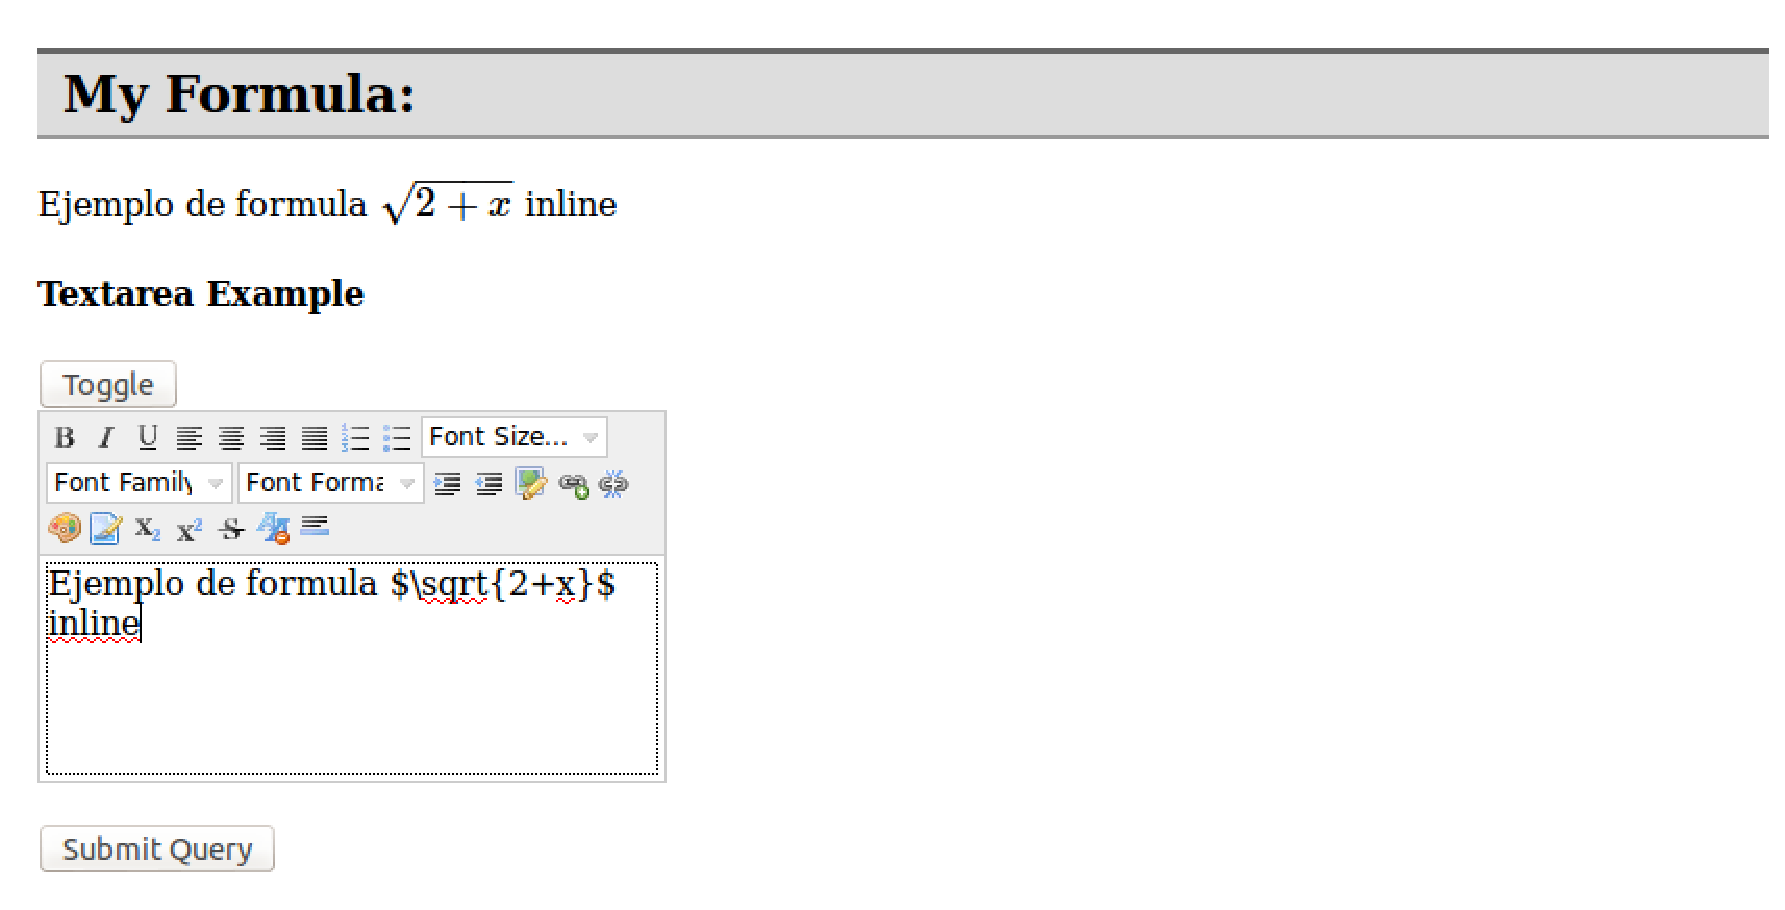
\includegraphics[width=0.9\textwidth]{fig/nax1}
  \caption{Prueba 1 : Nax Editor}
\end{figure}

Cabe destacar de esta primera propuesta su sencillez y calidad final demostrándose la facilidad con la que se integran ambas herramientas.

\subsection{NicEdit + WIRIS Plugin}
